
\section{RQ1. To what extent can we generate program variants for \wasm?}
\label{rq1}
This research question investigates whether we can artificially generate program variants for \wasm. Concretely, we use CROW to generate program variants from an original program, written in C/C++ or directly passing an LLVM bitcode module to it. Therefore, the first step and research question is related to the ability of CROW to generate a handful number of program variants. Our intuition is that the larger the number of generated variants, the better the program variants' security and reliability properties can offer.



\begin{figure*}[h]
    \centering
    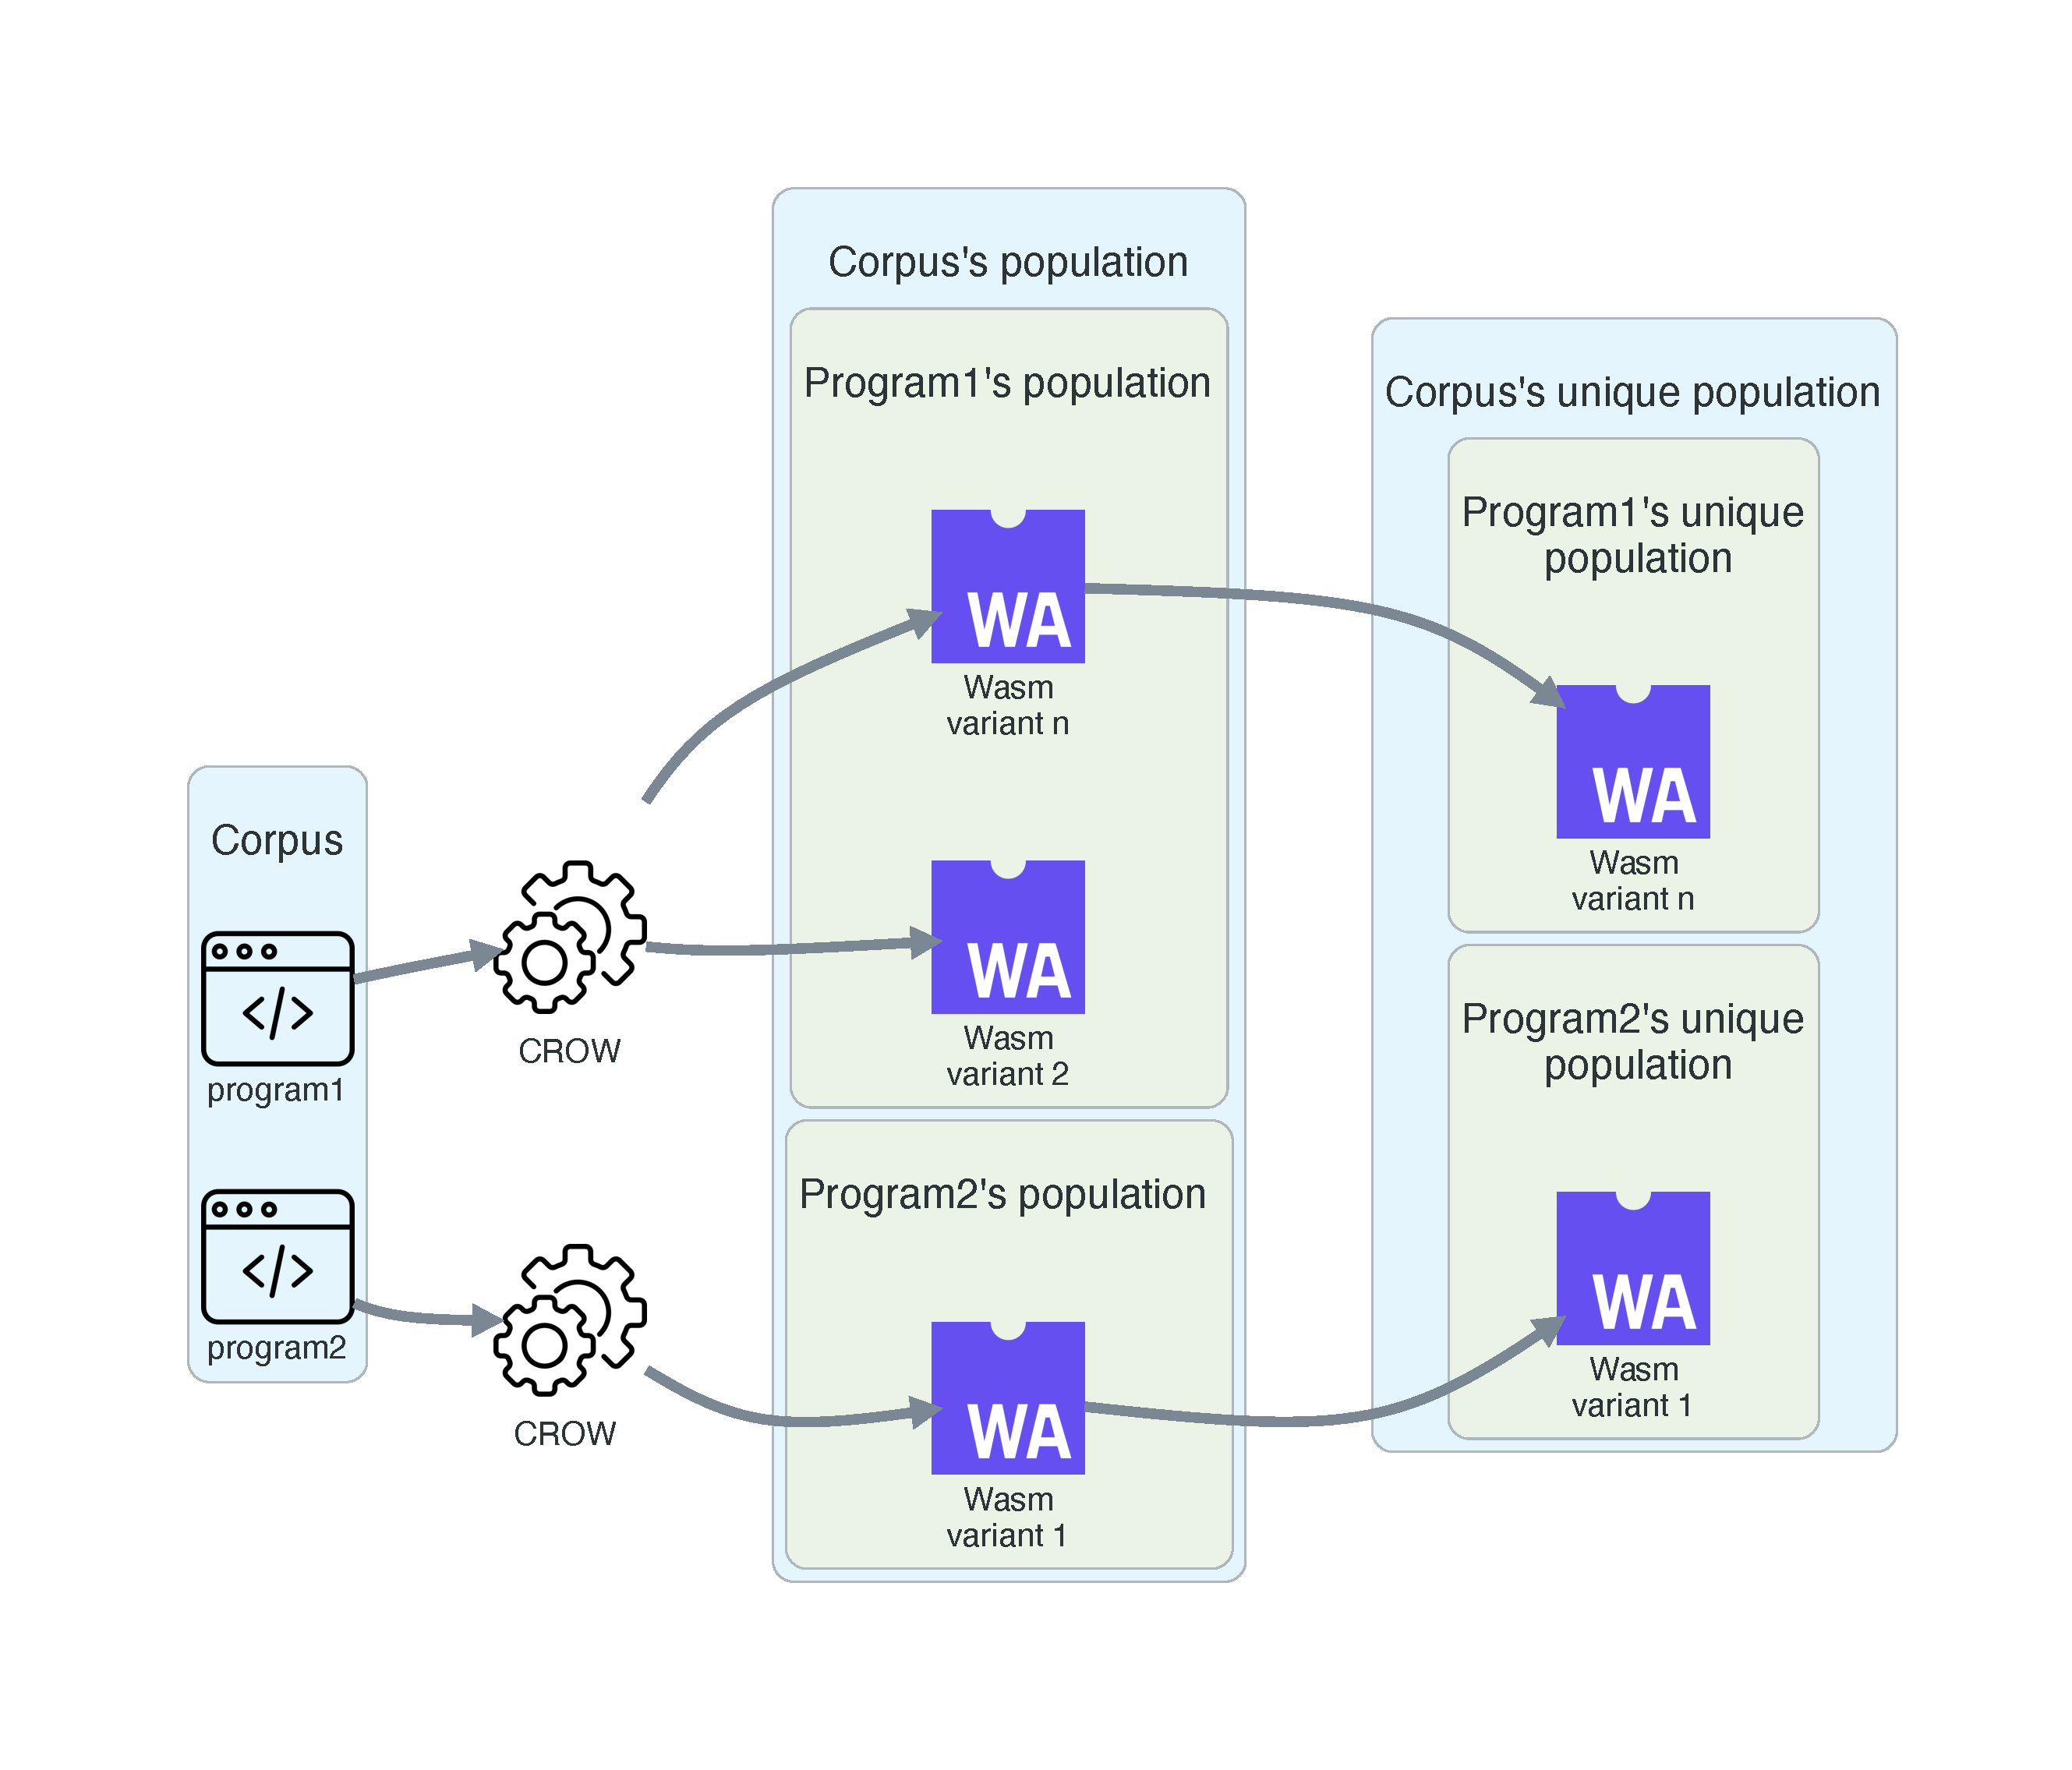
\includegraphics[height=2in]{diagrams/Rq1.pdf}
    \caption{Simplification of the program variants generation workflow.}
    \label{diagrams:protocol:rq1}
\end{figure*}


In \autoref{diagrams:protocol:rq1} we simplify the workflow to generate \wasm program variants. We pass each function of the corpora to CROW. To answer RQ1, we study the outcome of this pipeline, the generated variants. 

\subsection{Metrics}

To assess our approach's ability to generate \wasm binaries that are statically different, we compute the number of unique variants generated by CROW for each original function of each corpus. 



\begin{metric}{Population size $S(P)$:}\label{metric:md5sum}
    Given a program P and its generated variants $V$, the population size metric is defined as.\\
    $$
        S(P)=|V|
    $$

    Notice that, the variant population includes P as an instance.
\end{metric}

A program and its variants compose what we call a program's population. Notice that all proposed metrics over programs and their variants make sense only at the population level. Therefore, it only makes sense to compare semantically equivalent programs, i.e., from the same population. Along with this work, we use the term "program's population" to refer to a program and its variants.

\subsection{Protocol}



One design property of CROW is that all possible programs that can be generated for a given language (LLVM in this case) are constructed and verified for equivalence. Thus, there are two parameters to control the size of the search space and hence the time required to traverse it.
On the one hand, one can limit the size of the variants. On the other hand, one can limit the set of instructions used for the synthesis. In our experiments for RQ1, we use all the $60$ supported instructions in the synthesizer.

The former parameter allows us to find a trade-off between the number of variants that are synthesized and the time taken to produce them. For the current evaluation, given the size of the corpus, we set the exploration time to 1 hour maximum per function for \corpusrosetta. In the cases of \corpussodium\ and\ \corpusqrcode, we set the timeout to 5 minutes per function in the exploration stage. The decision behind the usage of lower timeout for \corpussodium
and \corpussodium is motivated by the properties listed in \autoref{table:corpora}. The latter two corpora are remarkably larger in terms of the number of instructions and functions count. 

We pass each of the $303 + \libsodiumfunctions + \qrcodefunctions$ functions in the corpora to CROW, as \autoref{diagrams:protocol:rq1} illustrates, to synthesize program variants. We then calculate \autoref{metric:md5sum} for each program's population and conclude by answering RQ1.
